\section{Experimentellt}
\label{sec:exper}
För att kunna analysera reaktionshastigheten behöver ni kunna följa
reaktionens gång som funktion av tid. Till ert förfogande kommer ni ha en
s.k. ``stopped-flow''-utrustning. Den fungerar enligt följande:

\begin{figure}[center]
  \centering
  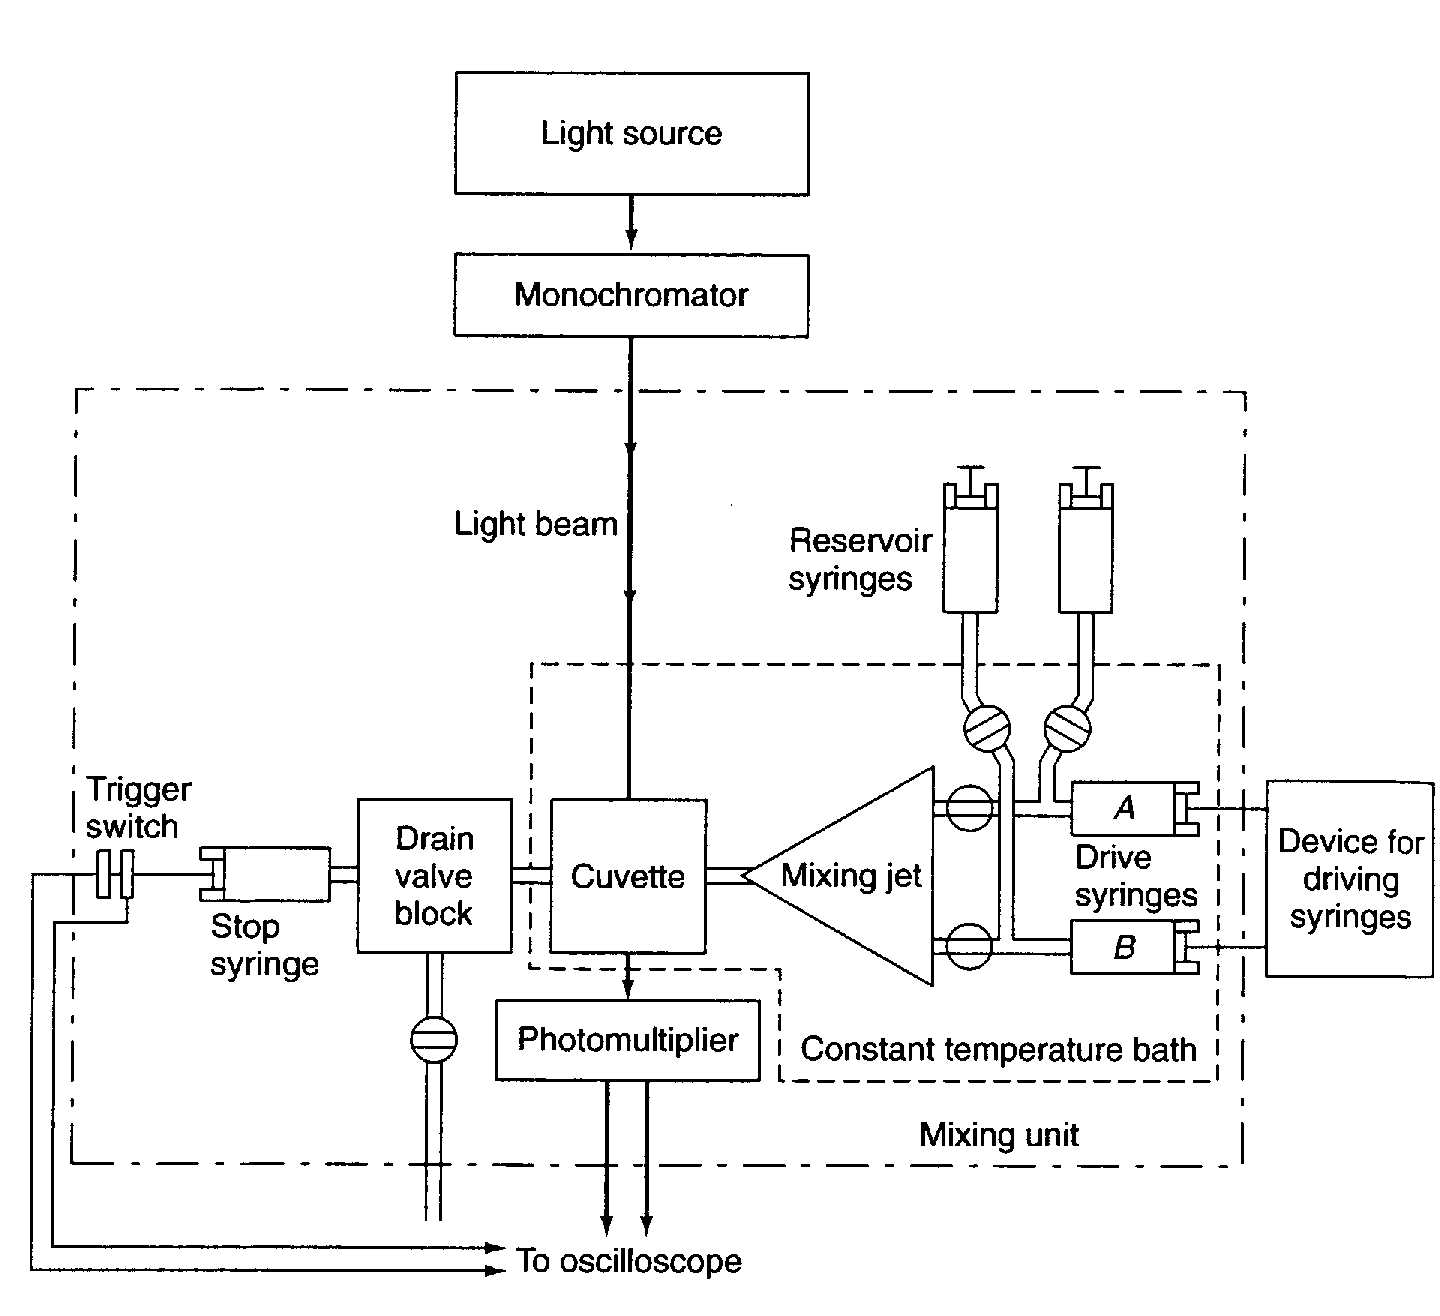
\includegraphics[scale=0.2]{fig/stopped_flow.png}
  \caption{Schematisk representation av stopped-flow utrustning}
  \label{fig:stopped-flow}
\end{figure}

Blandkammaren är termostaterad med hjälp av vattenbad som ni själva får
välja temperatur för. 

Istället för ett oscilloskåp kommer ni ha en dator med ett interface
skrivet i LabView. Från varje försök kommer ni att erhålla dataserier med
absorbans som funktion av tid vid en våglängd som ni själva väljer.


%%% Local Variables:
%%% mode: latex
%%% TeX-master: "../main"
%%% End:
